% !TEX program = lualatex

\documentclass{beamer}

\title{Modelos Generativos Profundos}
\subtitle{Clase 2: Repaso de conceptos previos}
\author{Fernando Fêtis Riquelme}
\institute{
    Facultad de Ciencias Físicas y Matemáticas\\
    Universidad de Chile
}
\date{Otoño, 2026}
\titlegraphic{\hfill
\includegraphics[height=1.2cm]{images/fcfm.pdf}}

\usetheme{metropolis}
\setbeamercovered{transparent}
\newcommand{\insertimage}[2]{%
\centering\includegraphics[width=#2\textwidth]{images/#1}\par
}
\renewcommand{\raggedright}{\leftskip=0pt \rightskip=0pt plus 0cm}
\newcommand{\R}{\mathbb{R}}
\newcommand{\N}{\mathbb{N}}

\begin{document}

\begin{frame}
    \titlepage
\end{frame}

\begin{frame}{Clase de hoy}
    \tableofcontents
\end{frame}

\section{Probabilidades}

\begin{frame}{Variables aleatorias}
    Una \textbf{v.a.} $x$ es una función que puede tomar distintos valores de acuerdo a una \textbf{distribución de probabilidad} $p(x)$.

    Dependiendo de la naturaleza de la v.a., $p(x)$ se interpreta de dos formas distintas:
    \begin{itemize}
        \item \textbf{Variable discreta:} $p(x)$ es una función de masa.
        \item \textbf{Variable continua:} $p(x)$ es una función de densidad.
    \end{itemize}
    El \textbf{soporte} de la v.a., $\text{supp}(x):=\{x:p(x)>0\}$, indica los distintos valores que una v.a. puede tomar.
\end{frame}

\begin{frame}{Variables aleatorias discretas}
    Si $x\sim p(x)$ es una v.a. discreta con $\text{supp}(x)=\{k_1,\ldots,k_N\}$, entonces su \textbf{función de masa} $p:\{k_1,\ldots,k_N\}\to[0,1]$ indica
    \begin{equation*}
        \text{Prob}(x=k_n)=p(k_n)
    \end{equation*}
    Por definición de medida de probabilidad, es necesario que:
    \begin{itemize}
        \item $p(k_n)\geq 0$, para todo $n\in\{1,\ldots,N\}$.
        \item $\sum_{n=1}^N p(k_n)=1$.
    \end{itemize}
\end{frame}

\begin{frame}{Variables aleatorias discretas}
    En el caso discreto se pueden almacenar todas las salidas de $p(x)$ en un \textbf{vector de probabilidades} $\left(p(k_1),\ldots,p(k_N)\right)\in[0,1]^N$.

    El conjunto de vectores de probabilidades de largo $N$ se denomina \textbf{$N$-símplex}:
    \begin{equation*}
        \hspace{-0.5cm}
        \Delta^N:=\left\{(p_1,\ldots,p_N)\in\R^N\,:\, \left(\sum_{n=1}^N p_n=1\right)\,\land\, \left(p_n\geq0,\,\forall n\in\{1,\ldots,N\}\right) \right\}
    \end{equation*}
\end{frame}

\begin{frame}{Distribución de Bernoulli}
    La distribución discreta más simple es la \textbf{distribución de Bernoulli}.

    Se dice que $x\sim \text{Bernoulli}(r)$, con $r\in[0,1]$, si $\text{supp}(x)=\{0,1\}$ con $\text{Prob}(x=1)=r$ y $\text{Prob}(x=0)=1-r$, i.e.:
    \begin{align*}
        p(x) & =\begin{cases}
                    r   & \text{si } x=1 \\
                    1-r & \text{si } x=0
                \end{cases}               \\
             & = r^x(1-r)^{1-x}, \quad x\in\{0,1\}
    \end{align*}
\end{frame}

\begin{frame}{Distribución categórica}
    La distribución de Bernoulli se puede extender al caso multiclase, dando lugar a la \textbf{distribución categórica}.

    Se dice que $x\sim\text{Categórica}(r)$, con $r\in\Delta^N$, si:
    \begin{itemize}
        \item $\text{supp}(x)=\{k_1,\ldots,k_N\}$.
        \item $\text{Prob}(x=k_n)=r_n$.
    \end{itemize}
    \insertimage{discrete}{1}
\end{frame}

\begin{frame}{Variables aleatorias continuas}
    Si $x\sim p(x)$ es una v.a. continua, su \textbf{función de densidad} $p:\R^D\to\R_+$ permite calcular la probabilidad de que $x$ esté en un cierto conjunto $A\subset\R^D$ mediante integración:
    \begin{equation*}
        \text{Prob}(x\in A)=\int_A p(x)\,\text{d}x
    \end{equation*}
    Por definición de medida de probabilidad, es necesario que:
    \begin{itemize}
        \item $p(x)\geq 0$, para todo $x\in\R^D$.
        \item $\int_{\R^D} p(x)\,\text{d}x=1$.
    \end{itemize}
    Notar que aquí no se cumple necesariamente que $p(x)\leq 1$.
\end{frame}

\begin{frame}{Distribución gaussiana}
    Para $\mu\in\R$ y $\sigma^2>0$, se dice que $x\sim\mathcal{N}(\mu,\sigma^2)$ es una v.a. \textbf{gaussiana} o \textbf{normal} (unidimensional) si tiene densidad
    \begin{equation*}
        p(x)=\frac{1}{\sqrt{2\pi\sigma^2}}\exp\left(-\frac{1}{2\sigma^2}(x-\mu)^2\right)
    \end{equation*}
    \insertimage{gaussian_1d}{1}
\end{frame}

\begin{frame}{Distribución gaussiana}
    La distribución gaussiana tiene las siguientes propiedades:
    \begin{itemize}
        \item Es una distribución unimodal de cola ligera.
        \item Si $x\sim\mathcal{N}(\mu,\sigma^2)$, entonces $ax+b\sim\mathcal{N}(a\mu+b,a^2\sigma^2)$.
        \item Si $x_1\sim\mathcal{N}(\mu_1,\sigma_1^2)$ y $x_2\sim\mathcal{N}(\mu_2,\sigma_2^2)$, entonces
              \begin{equation*}
                  x_1+x_2\sim\mathcal{N}(\mu_1+\mu_2,\sigma_1^2+\sigma_2^2)
              \end{equation*}
        \item $\log p(x)$ es una función cóncava.
        \item El promedio de v.a. i.i.d.s converge a una v.a. gaussiana.
        \item Es la distribución de máxima entropía dentro de la familia de distribuciones con soporte $(-\infty,\infty)$ y varianza finita.
    \end{itemize}
\end{frame}

\begin{frame}{Distribución gaussiana multivariada}
    Es posible extender la distribución gaussiana al caso multidimensional.

    Si $\mu=(\mu_1,\ldots,\mu_D)\in\R^D$ y $\Sigma\in\mathcal{M}_{D,D}(\R)$ es una matriz simétrica definida positiva, entonces $x\sim \mathcal{N}(\mu,\Sigma)$ si tiene densidad
    \begin{equation*}
        p(x)=\frac{1}{\sqrt{(2\pi)^D\text{det}(\Sigma)}}
        \exp\left(
        -\frac{1}{2}(x-\mu)^\top \Sigma^{-1}(x-\mu)
        \right)
    \end{equation*}
    \insertimage{gaussian_2d}{0.8}
\end{frame}

\begin{frame}{Distribución condicional y dependencia}
    Dadas dos v.a., $x\sim p(x)$ e $y\sim p(y)$, se denotará por $p(x|y)$ a la \textbf{distribución condicional} que sigue la v.a. $x$ cuando se conoce (o se fija) el valor que toma la v.a. $y$:
    \begin{equation*}
        p(x|y):=\frac{p(x,y)}{p(y)}
    \end{equation*}
    Las v.a. $x\sim p(x)$ e $y\sim p(y)$ se dicen \textbf{independientes} ($x\perp y)$ si
        \begin{equation*}
            p(x|y)=p(x)
            \quad\text{o, equivalentemente,}\quad
            p(x,y)=p(x)p(y)
        \end{equation*}
        La independencia es simétrica: si $x\perp y$, entonces $y\perp x$.

    Si dos v.a. no son independientes, se dicen \textbf{dependientes}.
\end{frame}

\begin{frame}{Marginalización}
    Dada una \textbf{distribución conjunta} $p(x,y)$, es posible obtener la distribución $p(x)$ mediante \textbf{marginalización}:
    \begin{align*}
        p(x) =\sum_{n=1}^N p(x,y=y_k)
        \quad\text{o bien}\quad
        p(x) = \int_{\R^D} p(x,y)\,\text{d}y
    \end{align*}
    \begin{figure}
        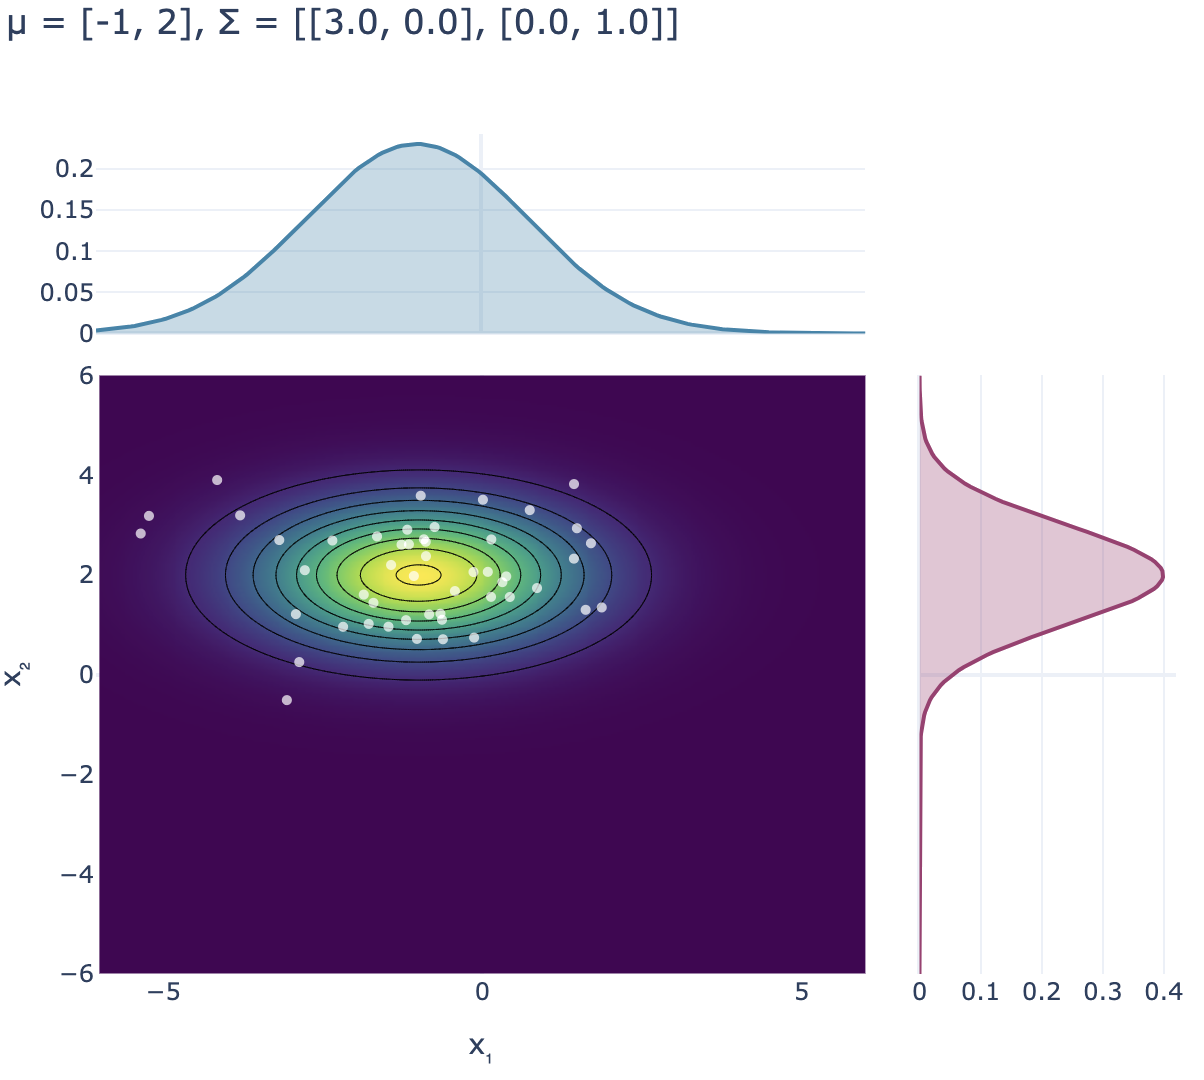
\includegraphics[width=0.35\textwidth]{images/marginal_1.png}
        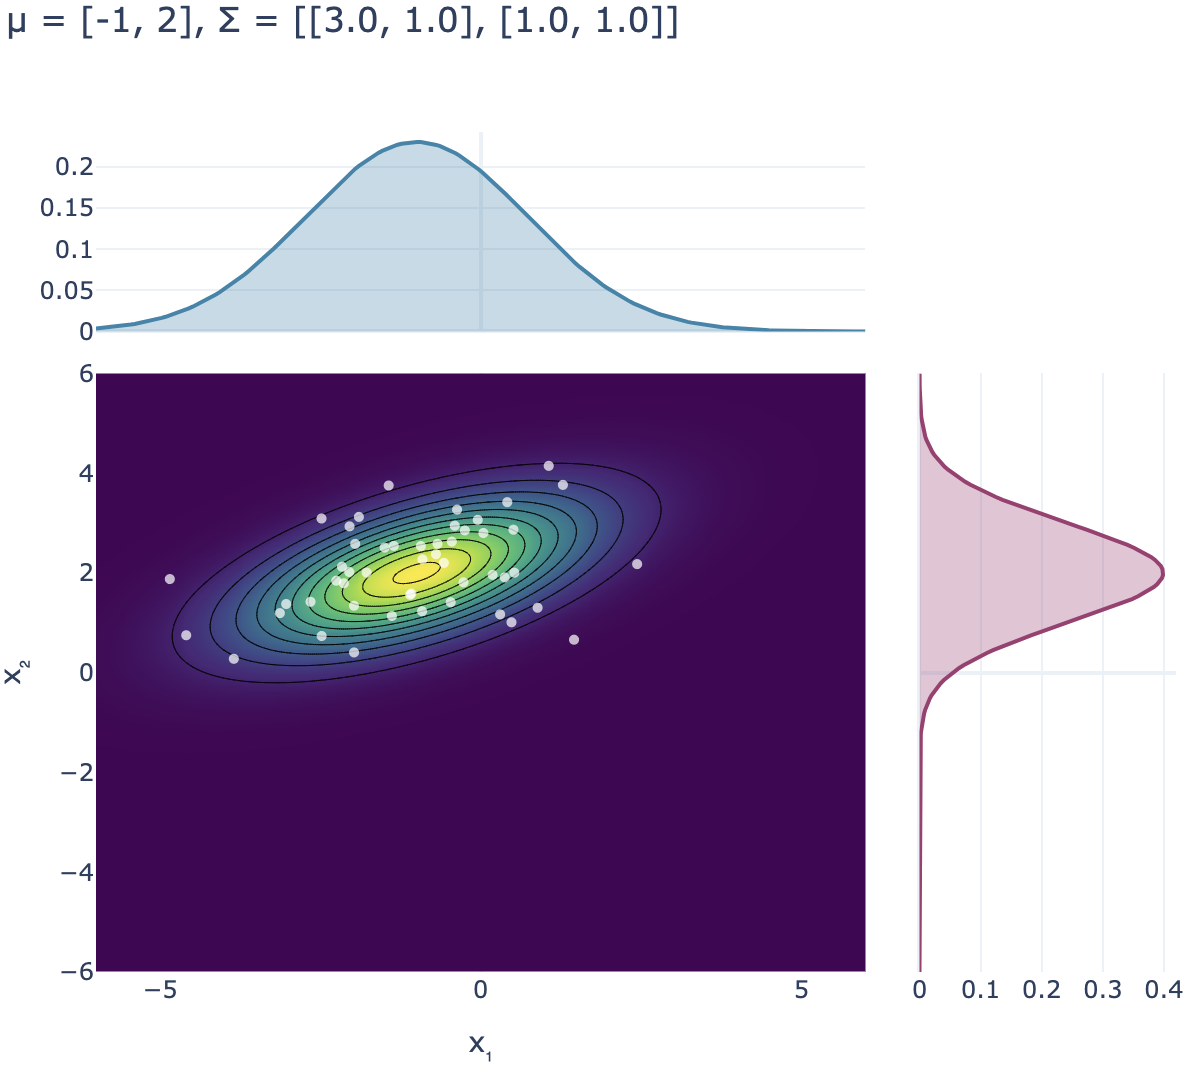
\includegraphics[width=0.35\textwidth]{images/marginal_2.png}
    \end{figure}
    Notar que la distribución conjunta $p(x,y)$ contiene más información que las distribuciones individuales $p(x)$ y $p(y)$.
\end{frame}

\begin{frame}{Regla de Bayes}
    Por definición de probabilidad condicional, es directo que
    \begin{equation*}
        p(y|x)=\frac{p(y)p(x|y)}{p(x)}
    \end{equation*}
    Este resultado se conoce como \textbf{regla de Bayes}.

    Esta propiedad se puede extender a un conjunto de variables aleatorias. Por inducción se prueba que
    \begin{align*}
        p(x_1,\ldots,x_N)=p(x_1)\prod_{n=2}^N p(x_n|x_1,\ldots,x_{n-1})
    \end{align*}
    Este resultado se conoce como \textbf{regla de la cadena}.
\end{frame}

\begin{frame}{Esperanza}
    Dada una v.a. $x\sim p(x)$, su \textbf{esperanza} corresponde al valor que se espera obtener al promediar muestras generadas desde $x$.

    Si $x\sim p(x)$ es una v.a. discreta con $\text{supp}(x)=\{k_1,\ldots,k_N\}$:
    \begin{equation*}
        \mathbb{E}_{x\sim p(x)}\left[x\right]:=\sum_{n=1}^N k_n\,p(k_n)
    \end{equation*}
    En general, para una función $f:\{k_1,\ldots,k_N\}\to\R$:
    \begin{equation*}
        \mathbb{E}_{x\sim p(x)}\left[f(x)\right]=\sum_{n=1}^N f(k_n)\, p(k_n)
    \end{equation*}
\end{frame}

\begin{frame}{Esperanza}
    En el caso continuo, la esperanza de una v.a. $x\sim p(x)$ se define de forma análoga:
    \begin{equation*}
        \mathbb{E}_{x\sim p(x)}\left[x\right]
        :=\int_{\R^D} x\, p(x)\,\text{d}x
    \end{equation*}
    De forma general, para $f:\R^D\to\R$:
    \begin{equation*}
        \mathbb{E}_{x\sim p(x)}\left[f(x)\right]
        =\int_{\R^D} f(x)\, p(x)\,\text{d}x
    \end{equation*}
    Por otro lado, se suele denotar $\mathbb{E}_{x\sim p(x)}\left[x\right]$ como $\mathbb{E}_{p(x)}\left[x\right]$ para no sobrecargar la notación.
\end{frame}

\begin{frame}{Esperanza}
    Si una v.a. no participa dentro del argumento, se puede omitir:
    \begin{align*}
        \mathbb{E}_{p(x,y)}[f(x)]=\mathbb{E}_{p(x)}[f(x)]
    \end{align*}
    Además, la esperanza es un operador lineal:
    \begin{align*}
        \mathbb{E}_{p(x,y)}[\alpha x+\beta y]
        =\alpha\,\mathbb{E}_{p(x)}[x] + \beta\,\mathbb{E}_{p(y)}[y]
    \end{align*}
    Por otro lado, la esperanza se puede factorizar de forma similar a la distribución conjunta:
    \begin{align*}
        \mathbb{E}_{p(x,y)}[f(x,y)] =
        \mathbb{E}_{p(y)}\left[\mathbb{E}_{p(x|y)}[f(x,y)]\right]
    \end{align*}
\end{frame}

\begin{frame}{Esperanza}
    Si $x\sim p(x)$ es una v.a. desde la cual es fácil generar muestras, la ley de grandes números permite aproximar una esperanza:
    \begin{equation*}
        \mathbb{E}_{p(x)}[f(x)]\approx \frac{1}{N}\sum_{n=1}^N f(x^n),
    \end{equation*}
    donde $x^n\sim p(x)$ para todo $n\in\{1,\ldots,N\}$.

    Esta aproximación se suele llamar \textbf{estimación de Monte Carlo}.
\end{frame}

\begin{frame}{Varianza y covarianza}
    La \textbf{varianza} de una v.a. $x\sim p(x)$ en $\R$ corresponde a la desviación cuadrática media de la v.a. con respecto a su media $\mu=\mathbb{E}_{p(x)}\left[x\right]$:
    \begin{align*}
        \text{Var}(x):=\mathbb{E}_{p(x)}\left[(x-\mu)^2\right]
    \end{align*}
    Este concepto se puede extender al concepto de covarianza. Si $x\sim p(x)$ e $y\sim p(y)$ son dos v.a. en $\R$ con medias $\mu_x$ y $\mu_y$:
    \begin{equation*}
        \text{Cov}(x,y):=\mathbb{E}_{p(x,y)}\left[(x-\mu_x)(y-\mu_y)\right]
    \end{equation*}
    En particular, $\text{Cov}(x,x)=\text{Var}(x)\geq 0$.
\end{frame}

\begin{frame}{Varianza y covarianza}
    Notar que $\text{Cov}(x,y)=0$ no implica necesariamente que $x\perp y$ ya que la covarianza solo puede captar relaciones lineales entre las variables.

    Cuando se tiene una v.a. $x=(x_1,\ldots,x_D)\sim p(x)$ en $\R^D$, es posible construir su \textbf{matriz de covarianzas}, $\text{Cov}(x)\in\mathcal{M}_{D,D}(\R)$:
    \begin{equation*}
        \text{Cov}(x)_{ij}:=\text{Cov}(x_i,x_j)
    \end{equation*}
    En particular, la diagonal de esta matriz contiene las varianzas de cada componente de $x$.

    Notando que $\text{Cov}(x_i,x_j)=\text{Cov}(x_j,x_i)$, se tiene que la matriz de covarianzas siempre es simétrica.
\end{frame}

\section{Redes neuronales}

\begin{frame}{Formulación}
    Una \textbf{red neuronal} es una función \textit{adaptable} $f:\R^D\to\R^C$ que se puede \textbf{entrenar} para replicar el comportamiento de otra función $f_\text{data}:\R^D\to\R^C$ desconocida.

    Para esto, se utiliza un \textbf{conjunto de entrenamiento}
    \begin{equation*}
        \mathcal{D}=\left\{(x^1,y^1),\ldots,(x^N,y^N)\right\}\subset\R^D\times\R^C,
    \end{equation*}
    donde cada instancia $(x^n,y^n)\in\mathcal{D}$ es de la forma $y^n=f_\text{data}(x^n)$.

    De este modo, cuando la red neuronal $f$ está entrenada,
    \begin{equation*}
        f(x^n)\approx f_\text{data}(x^n)
        \quad\text{para todo}\quad
        n\in\{1,\ldots,N\}.
    \end{equation*}
\end{frame}

\begin{frame}{Formulación}
    Una red neuronal está formada por la composición de $K\in\N$ funciones individuales, $f_k:\R^{D_{k-1}}\to\R^{D_k}$ (con $D_0=D$ y $D_K=C$):
    \begin{equation*}
        f(x)=f_K(f_{K-1}(...(f_1(x))...))
    \end{equation*}
    Cada \textbf{capa} $f_k$ tiene tiene asociado un conjunto de \textbf{parámetros} $\theta_k\in\R^{P_k}$ que van cambiando durante el entrenamiento.

    Se pueden concatenar los $K$ parámetros en un único vector $\theta\in\R^P$, con $P=\sum_{k=1}^K P_k$, lo que motiva a usar la notación $f_\theta$.

    Las redes neuronales serán, por lo general, usadas para ajustar los parámetros de una distribución de probabilidad.
\end{frame}

\begin{frame}{Entrenamiento}
    Para entrenar una red neuronal es necesario elegir una \textbf{función de pérdida} $L:\R^C\times\R^C\to\R$.

    Esta función mide la discrepancia entre el valor real y el valor predicho por la red neuronal para una instancia $(x^n,y^n)\in\mathcal{D}$.

    De esta forma, la función de pérdida total sobre el conjunto de entrenamiento $\mathcal{D}=\left\{(x^1,y^1),\ldots,(x^N,y^N)\right\}\subset\R^D\times\R^C$ es:
    \begin{equation*}
        \mathcal{L}_\mathcal{D}\left(\theta\right)=\frac{1}{N}\sum_{n=1}^N L\left(f_\theta(x^n),y^n\right)
    \end{equation*}
\end{frame}

\begin{frame}{Entrenamiento}
    Para entrenar una red neuronal se deben ajustar sus parámetros de tal forma que minimicen el valor de $\mathcal{L}_\mathcal{D}\left(\theta\right)$.

    Para esto, lo más usual es usar \textbf{algoritmos de gradiente}, los cuales realizan iteraciones de la forma
    \begin{equation*}
        \theta\leftarrow\theta - \gamma\,\nabla_{\theta} \mathcal{L}_\mathcal{D}\left(\theta\right),
    \end{equation*}
    donde la constante $\gamma>0$ se llama \textbf{tasa de aprendizaje}.

    Todos los optimizadores usados necesitan conocer $\nabla_\theta \mathcal{L}_\mathcal{D}\left(\theta\right)$, lo cual es obtenido mediante \textbf{backpropagation}.
\end{frame}

\begin{frame}{Redes fully connected}
    El tipo de red neuronal más simple es la red \textbf{fully connected}, donde cada capa $f_k:\R^{D_{k-1}}\to\R^{D_k}$ es de la forma
    \begin{equation*}
        f_k(x)=\Phi(A_kx+b_k),
    \end{equation*}
    con $A_k\in\mathcal{M}_{D_k,D_{k-1}}(\R)$ y $b_k\in\R^{D_k}$ los parámetros de $f_k$.

    La función $\Phi:\R^{D_k}\to\R^{D_k}$ suele ser una misma función que se aplica en cada coordenada del vector de \textbf{pre-activación}:
    \begin{equation*}
        \Phi(y)=\left(\phi(y_1),\ldots,\phi(y_{D^k})\right),
    \end{equation*}
    donde $\phi:\R\to\R$ es una función no lineal fija llamada \textbf{función de activación}.
\end{frame}

\begin{frame}{Redes neuronales con múltiples entradas}
    Las redes neuronales pueden ser modificadas para que reciban información adicional (p.g. un prompt o una imagen).

    Para esto, se puede sustituir cada capa $f_k:\R^{D_{k-1}}\to\R^{D_k}$ por otra capa $f_k:\R^{D_{k-1}}\times\R^J\to\R^{D_k}$ que sea capaz de procesar un contexto adicional $c\in\R^J$.

    Una forma simple de hacer esto en una red FC es la siguiente:
    \begin{equation*}
        f_k(x,c)=\Phi(A_kx+B_kc+d_k),
    \end{equation*}
    donde $A_k\in\mathcal{M}_{D_k,D_{k-1}}(\R)$, $B_k\in\mathcal{M}_{D_k,J}(\R)$ y $d_k\in\R^{D_k}$ son los parámetros de la nueva capa $f_k$.
\end{frame}

\begin{frame}{Clasificación con redes neuronales}
    Si $\mathcal{D}=\left\{(x^1,y^1),\ldots,(x^N,y^N)\right\}$ es un dataset compuesto por pares de imágenes y etiquetas de clase, se puede ajustar un modelo probabilístico para predecir la clase $y\in\{M_1,\ldots,M_C\}$ a la que pertenece una imagen $x\in\R^D$ dada:
    \begin{equation*}
        p_\theta(y|x)\sim\text{Categórica}(r_\theta(x)),
    \end{equation*}
    con $r_\theta:\R^D\to\Delta^C$ una red neuronal que mapea cada imagen $x\in\R^D$ a un vector de probabilidades $r_\theta(x)\in\Delta^C$ sobre las clases.
\end{frame}

\begin{frame}{Clasificación con redes neuronales}
    La salida de la red neuronal $r_\theta:\R^D\to\Delta^C$ debe ser un vector de probabilidades.

    Para esto, se suele usar la función de activación $\text{softmax}:\R^C\to\Delta^C$ en la última capa:
    \begin{equation*}
        \text{softmax}(s):=\left(\frac{e^{s_1}}{\sum_{c=1}^C e^{s_c}}, \ldots,\frac{e^{s_C}}{\sum_{c=1}^C e^{s_c}}\right)
    \end{equation*}
    Como función de pérdida se suele usar la \textbf{entropía cruzada}, la cual será revisada en más detalle al estudiar redes bayesianas.
\end{frame}

\begin{frame}{Próxima clase}
    En la próxima clase.
    \begin{itemize}
        \item Introducción a las redes bayesianas.
        \item Modelos generativos modernos como redes bayesianas.
    \end{itemize}
\end{frame}

\begin{frame}
    \centering
    \Large{Modelos Generativos Profundos}\\
    \large{Clase 2: Repaso de conceptos previos}
\end{frame}

\end{document}
